\chapter{Analýza}
\label{sec:an}

\section{Struktura systému}

Struktura celého systému je naznačena na obrázku \ref{fig:basic_struct}. Podřízené systémy komunikují s~nadřazeným na základě událostí. Nadřazený systém tyto události zpracovává a upravuje podle nich stav garáží v~evidenci. 

Zaznamenané události jsou také uchovávány v~historii událostí, spolu s~dalšími metadaty jako čas přijetí nebo původce.

%Komunikace mezi podřízeným a nadřazeným systémem je postavena na modelu klient-server. Nadřazený systém tedy provozuje server zvoleného protokolu, ke kterému se podřízené systémy připojují. %tohle sem pridat kdyz mi potvrdi klient/server model, jinak napsat ze subscriber/publisher, s tim ze garaze i system sou publisheri

Další, kdo přistupuje do systému, je uživatel. Přes webové rozhraní může sledovat stav garáží a historii událostí. Také zde může spravovat klíče, které slouží pro přístup ke komunikačnímu API systému. Přístup do webového rozhraní je zabezpečen heslem. 

\begin{figure}[h!]
    \centering
    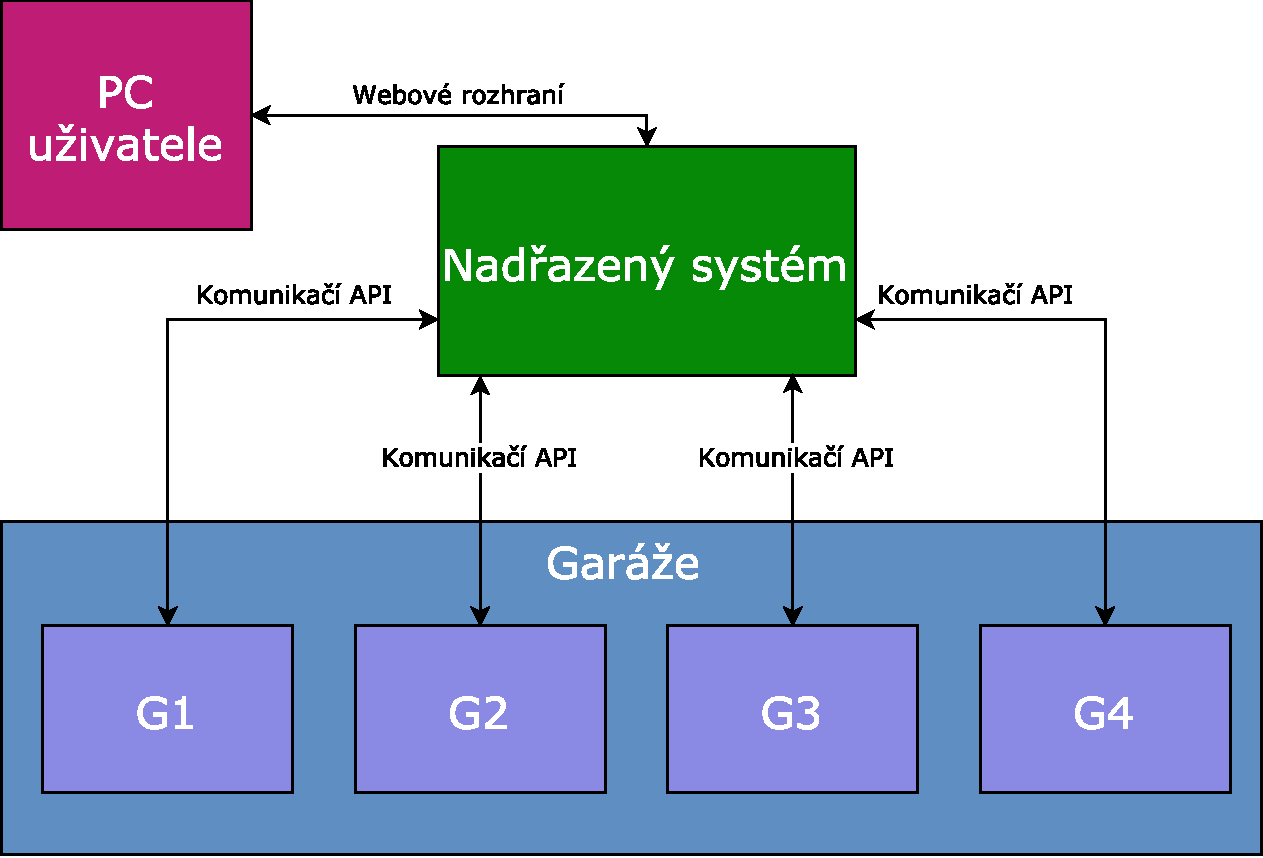
\includegraphics[width=0.7\textwidth]{images/basic_struct.pdf}
    \label{fig:basic_struct}
    \caption{Základní struktura systému}
\end{figure}

\subsection{Podřízený systém}

Podřízený systém je zařízení umístěné v~každé garáži, které sleduje stav okolí pomocí těchto senzorových vstupů:

\begin{itemize}
    \item teplota,
    \item světelá intenzita (fotobuňka),
    \item detekce kouře,
    \item detekce pohybu,
    \item stav dveří.
\end{itemize}

V~případě překročení mezních hodnot se zařízení okamžitě hlásí nadřazenému systému. Kromě toho také v~pravidelných intervalech odesílá kontrolní hlášení. 

Vyhodnocení události je provedeno nadřazeným systémem. Podřízený systém tedy hlásí každou událost (například otevření dveří), aniž by nějak zkoumal její závažnost.

Základní požadavek na podřízený systém je schopnost komunikace přes Ethernet či WiFi pomocí protokolu zvoleného v~sekci \ref{sec:an_protocol}. Kromě toho může být hardware prakticky libovolný.

\section{Výběr komunikačního protokolu}
\label{sec:an_protocol}

Nejdřív je nutné určit způsob komunikace, který bude systém používat. Díky tomu se budu při vybíraní platformy moci ujistit, že jsou dostupné vhodné knihovny a další software. 

Nadřazený systém bude se svými klienty (monitorovací zařízení v~jednotlivých garážích) komunikovat přes WiFi nebo Ethernet. Základem komunikace bude TCP/IP protokol, je však potřeba zvolit vhodný protokol z~aplikační vrstvy OSI modelu, který na něm bude stavět.

\subsection{Vlastní protokol}

Jedna z~možností je implementovat vlastní protokol pomocí TCP/IP socketů. Toto řešení se mi však nezdá příliš vhodné, neboť nepřináší žádné významné výhody, naopak se s~ním pojí řada komplikací.

Pro vlastní protokol by bylo nutné vytvořit robustní server, který zvládá obsluhu více klientů najednou. Dále by vzhledem k~citlivosti přenášených dat bylo nutné implementovat nějakou formu šifrování. Tyto velmi obsáhlé problémy přitom řeší většina dnešních protokolů.

Další nevýhodou je nutnost implementace klientské části protokolu při vytváření nových zařízení spravovaných nadřazeným systémem. To do jisté míry omezuje jeho rozšiřitelnost.

\subsection{HTTPS}

Další možnost je využít ke komunikaci protokol HTTPS. V~tomto případě by klienti komunikovali se sytémem pomocí HTTP metod jako například \verb|get| nebo \verb|post|.

Jelikož součástí požadavků na systém je i webové uživatelské rozhraní, bude v~každém případě nutné použít webový server pro jeho provoz. Ten by pak bylo možné využít i k~poskytnutí API pro komunikaci systému s~garážovými čidly.

Vhodný webový server (jako například \textit{Nginx}) zajistí vícevláknovou obsluhu všech klientů. Protokol se také postará o~kryptografické zabezpeční přenášených dat, je však nutné získat certifikát k~ověření pravosti serveru (viz sekce \ref{an_certs}). 

API realizované pomocí tohoto protokolu je poměrně snadno rozšiřitelné. Pro nově implementovanou operaci stačí definovat URL a případně formát přenášených dat.

Výhodou je také snadná implementace na straně klienta, tedy garážového čidla. Knihovny realizující klientskou část protokolu jsou dostupné na většině populárních platforem jako například \textit{Arduino} (s~Ethernet shieldem, oficiální knihovna \textit{EthernetClient} \cite{ard_web}) nebo \textit{ESP8266} (knihovna \textit{esp8266wifi} \cite{esp_web}).

\subsubsection{Certifikáty pro provoz HTTPS}
\label{an_certs}

Pro provoz HTTPS serveru lze použít například certifikáty nadace Let's Encrypt, které jsou poskytovány  zdarma. Kromě toho dodává Let's Encrypt také automatizačního klienta \textit{Certbot} \cite{certbot} pro snadné nasazení a aktualizaci jejich certifikátů. Bohužel certifikáty jsou vydávány pouze na doménu \cite{lets_encrypt_faq}, což by značně komplikovalo nasazení zařízení v~místní síti.

Jiná možnost je použití \textit{self-signed} certifikátu.

Certifikát bude potřeba zajistit i v~případě, že komunikace s~klienty nebude postavena na tomto protokolu. Je totiž nutné také zabezpečit webové rozhraní, například kvůli ověření identity uživatele. Nutnost pořízení certifikátu tedy nepředstavuje nevýhodu oproti jiným protokolům.

\subsection{MQTT}

\cite{mqtt_valerie}

\section{Výběr platformy}

Pro realizaci systému je nutné zvolit vhodnou platformu. Jelikož je cílem práce vytvořit fyzické zařízení, rozhodl jsem se jako základ použít některý z~jednodeskových počítačů, které jsou v~dnešní době na trhu. Tyto počítače bývají cenově velmi dostupné a zároveň poskytují dostatečný výkon a podporu pro provoz systému.

Při výběru počítače byla nejdůležitejším kritériem podpora softwaru potřebného k~implementaci monitorovacího systému.